\documentclass[12pt]{article}
\usepackage[a4paper,margin=1in]{geometry}
\usepackage{amsmath}
\usepackage{amssymb}
\usepackage{enumitem}
\usepackage{tikz}
\usetikzlibrary{
    arrows.meta,
    calc,
    angles,
    quotes,
    decorations.pathmorphing
}
\usepackage[american]{circuitikz}



\begin{document}

\begin{enumerate}

\item A particle moves along the x-axis under acceleration $(a = kx)$ with $(k>0)$, starting from rest at $(x=x_0)$. When it reaches $(x=\frac{3}{2}x_0)$, the constant changes to $(k(1+\varepsilon))$ with $(\varepsilon\ll1)$, and motion continues without impulse. Neglecting $(\varepsilon^2)$ terms, find the speed when it reaches $(x=2x_0)$.

\begin{enumerate}[label=\Alph*)]
\item $(\sqrt{3k x_0^2}\left(1+\frac{\varepsilon}{6}\right))$
\item $(\sqrt{3k x_0^2}\left(1+\frac{\varepsilon}{3}\right))$
\item $(\sqrt{2k x_0^2}\left(1+\frac{\varepsilon}{6}\right))$
\item $(\sqrt{3k x_0^2}\left(1-\frac{\varepsilon}{6}\right))$
\end{enumerate}

\item A block of mass $(m)$ slides down a smooth wedge of mass $(M)$ on a smooth horizontal surface, wedge angle $(\theta)$. During motion gravity changes to $(g(1-\varepsilon))$, $(\varepsilon\ll1)$, without altering constraints. Using horizontal momentum conservation and relative acceleration geometry, determine the wedge acceleration to first order in $(\varepsilon)$.
% ===============================
% DIAGRAM FOR QUESTION 2
% Block on Wedge (Mass M) on Smooth Surface
% ===============================



\begin{center}
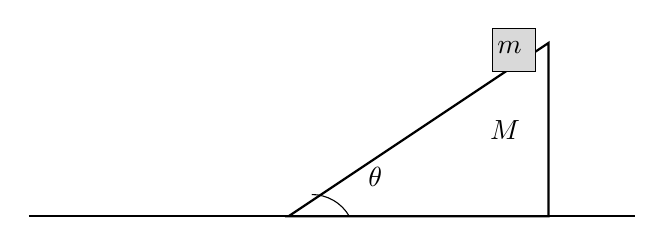
\begin{tikzpicture}[scale=1.1]

% Ground
\draw[thick] (-3,0) -- (4,0);

% Wedge
\draw[thick] (0,0) -- (3,0) -- (3,2) -- cycle;

% Block
\draw[fill=gray!30] (2.35,2.17) rectangle (2.85,1.67);

% Angle
\draw (3,0) -- ++(-0.6,0);
\draw (.7,0) arc (30:90:0.5);
\node at (1,0.45) {$\theta$};

% Labels
\node at (2.5,1) {$M$};
\node at (2.55,1.95) {$m$};

\end{tikzpicture}
\end{center}


\begin{enumerate}[label=\Alph*)]
\item $\left(\frac{mg\sin\theta\cos\theta}{M+m\sin^2\theta}(1-\varepsilon)\right)$
\item $\left(\frac{mg\sin\theta\cos\theta}{M+m\sin^2\theta}\left(1-\varepsilon\frac{M}{M+m\sin^2\theta}\right)\right)$
\item $\left(\frac{mg\sin\theta\cos\theta}{M+m\sin^2\theta}\left(1-\varepsilon\frac{m\sin^2\theta}{M+m\sin^2\theta}\right)\right)$
\item $\left(\frac{mg\sin\theta\cos\theta}{M+m\sin^2\theta}\right)$
\end{enumerate}

\item Two masses $(m)$ and $(2m)$ are connected over a smooth pulley, initially at rest. After descending distance $(h)$, gravity increases to $(g(1+\varepsilon))$ with $(\varepsilon\ll1)$. Using coupled Newton equations before and after the change, find the new tension immediately after the change to first order in $(\varepsilon)$.

% ===============================
% DIAGRAM FOR QUESTION 3
% Atwood Machine
% ===============================



\begin{center}
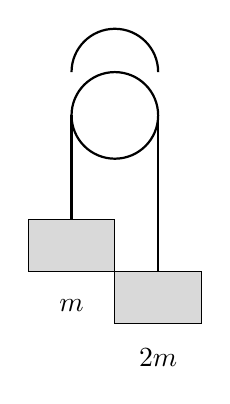
\begin{tikzpicture}[scale=1.1]

% Pulley
\draw[thick] (0,2) circle (0.5);
\draw[thick] (-0.5,2.5) arc (180:0:0.5);

% Strings
\draw[thick] (-0.5,2) -- (-0.5,0.8);
\draw[thick] (0.5,2) -- (0.5,0.2);

% Masses
\draw[fill=gray!30] (-1,0.2) rectangle (0,0.8);
\node at (-0.5,-0.2) {$m$};

\draw[fill=gray!30] (0, -0.4) rectangle (1,0.2);
\node at (0.5,-0.8) {$2m$};

\end{tikzpicture}
\end{center}

\begin{enumerate}[label=\Alph*)]
\item $\left(\frac{4mg}{3}(1+\varepsilon)\right)$
\item $\left(\frac{4mg}{3}\left(1+\frac{2\varepsilon}{3}\right)\right)$
\item $\left(\frac{4mg}{3}\left(1+\frac{\varepsilon}{3}\right)\right)$
\item $\left(\frac{4mg}{3}\right)$
\end{enumerate}

\item A projectile of fixed speed $(u)$ is projected at varying angles such that all trajectories pass through a fixed point $((x_0,y_0))$. The envelope of trajectories is formed by eliminating angle; if speed increases to $(u(1+\varepsilon))$, determine the new equation of envelope to first order in $(\varepsilon)$.

\begin{enumerate}[label=\Alph*)]
\item $\left(y=\frac{u^2}{2g}(1+2\varepsilon)-\frac{g x^2}{2u^2}(1-2\varepsilon)\right)$
\item $\left(y=\frac{u^2}{2g}(1+\varepsilon)-\frac{g x^2}{2u^2}(1-\varepsilon)\right)$
\item $\left(y=\frac{u^2}{2g}-\frac{g x^2}{2u^2}\right)$
\item $\left(y=\frac{u^2}{2g}(1+\varepsilon)-\frac{g x^2}{2u^2}(1-2\varepsilon)\right)$
\end{enumerate}

\item A particle of mass $(m)$ moves under central force $(F=-kr)$ and initially describes a circular orbit of radius $(R)$ with angular frequency $(\omega_0)$. The force constant is slowly increased to $(k(1+\varepsilon))$, $(\varepsilon\ll1)$, while angular momentum remains conserved and motion readjusts to a new circular orbit. Neglecting $(\varepsilon^2)$ terms, determine the new angular frequency in terms of $(\omega_0)$.

\begin{enumerate}[label=\Alph*)]
\item $\left(\omega_0\left(1+\varepsilon\right)\right)$
\item $\left(\omega_0\left(1+\frac{\varepsilon}{2}\right)\right)$
\item $\left(\omega_0\left(1+\frac{3\varepsilon}{2}\right)\right)$
\item $\left(\omega_0\left(1-\frac{\varepsilon}{2}\right)\right)$
\end{enumerate}

\item A uniform chain of length $(L=2,\text{m})$ just begins to slide off a smooth table with negligible overhang. Using exact energy redistribution between moving and falling segments, determine the speed (in m/s) when the chain completely leaves the table, taking $(g=10,\text{m/s}^2)$.

\begin{enumerate}[label=\Alph*)]
\item 4.47
\item 3.16
\item 2.58
\item 5.16
\end{enumerate}

\item A block of mass $(1,\text{kg})$ with speed $(4,\text{m/s})$ slides on a rough horizontal surface with $(\mu=0.2)$ and compresses a spring of constant $(800,\text{N/m})$; during compression friction acts throughout and $(g=10,\text{m/s}^2)$. Solving the coupled work--energy equation including friction over compression distance, maximum compression (in cm) is approximately:

\begin{enumerate}[label=\Alph*)]
\item 8.0
\item 8.9
\item 10.0
\item 7.2
\end{enumerate}

\item A particle of mass $(2,\text{kg})$ moves under constant power $(P=8,\text{W})$ starting from rest; using $(P=Fv)$ and integrating the nonlinear velocity equation exactly, determine its speed (in m/s) at $(t=4,\text{s})$.

\begin{enumerate}[label=\Alph*)]
\item 4.0
\item 3.2
\item 2.0
\item 5.6
\end{enumerate}

\item Two particles of masses $(1,\text{kg})$ and $(2,\text{kg})$ collide elastically in one dimension, heavier initially at rest; lighter approaches with $(6,\text{m/s})$. Using simultaneous conservation of momentum and kinetic energy without shortcut formulae, determine final velocity of lighter mass (in m/s).

\begin{enumerate}[label=\Alph*)]
\item -2
\item -4
\item 2
\item 4
\end{enumerate}

\item A block of mass $(2,\text{kg})$ slides down a smooth wedge of mass $(3,\text{kg})$ placed on a smooth horizontal surface, wedge angle $(30^\circ)$, $(g=10,\text{m/s}^2)$. Using horizontal momentum conservation and constraint acceleration components simultaneously, determine acceleration of wedge (in m/s$^2$).

% ===============================
% DIAGRAM FOR QUESTION 10
% Block on Wedge (Numerical Version)
% ===============================



\begin{center}
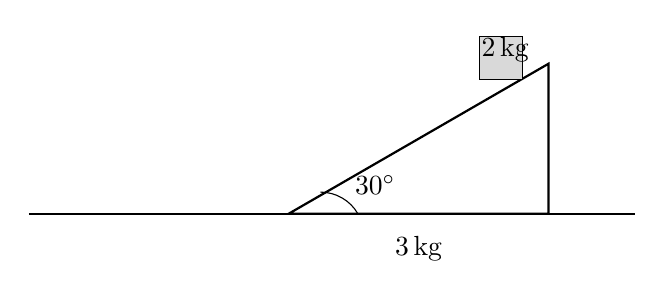
\begin{tikzpicture}[scale=1.1]

% Ground
\draw[thick] (-3,0) -- (4,0);

% Wedge
\draw[thick] (0,0) -- (3,0) -- (3,1.732) -- cycle;

% Block
\draw[fill=gray!30] (2.2,2.05) rectangle (2.7,1.55);

% Angle marking
\draw (.8,0) arc (30:90:0.5);
\node at (1,0.33) {$30^\circ$};


% Labels
\node at (1.5,-0.4) {$3\,\text{kg}$};
\node at (2.5,1.9) {$2\,\text{kg}$};

\end{tikzpicture}
\end{center}

\begin{enumerate}[label=\Alph*)]
\item 1.73
\item 2.00
\item 1.25
\item 2.50
\end{enumerate}

\item A uniform rod of length $(L=1,\text{m})$ and mass $(2,\text{kg})$ is hinged at one end and released from horizontal position under gravity $(g=10,\text{m/s}^2)$. Using rotational energy conservation about hinge and parallel-axis theorem consistently, determine angular speed (in rad/s) when rod becomes vertical.

% ===============================
% DIAGRAM FOR QUESTION 11
% Hinged Rod
% ===============================



\begin{center}
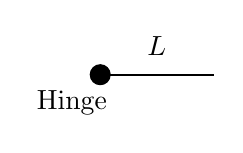
\begin{tikzpicture}[scale=1.2]

% Hinge
\filldraw (0,0) circle (3pt);

% Rod (initial horizontal)
\draw[thick] (0,0) -- (1.2,0);

% Label
\node at (0.6,0.3) {$L$};
\node at (-0.3,-0.3) {Hinge};

\end{tikzpicture}
\end{center}

\begin{enumerate}[label=\Alph*)]
\item 5.48
\item 4.47
\item 6.32
\item 3.16
\end{enumerate}

\item A particle of mass $(1,\text{kg})$ is attached to a light string of length $(1,\text{m})$ and is projected horizontally from lowest point with speed $(6,\text{m/s})$, $(g=10,\text{m/s}^2)$. Using simultaneous radial force balance and energy conservation, determine tension in string (in N) when particle reaches $(60^\circ)$ from lowest point.

% ===============================
% DIAGRAM FOR QUESTION 12
% Vertical Circle
% ===============================



\begin{center}
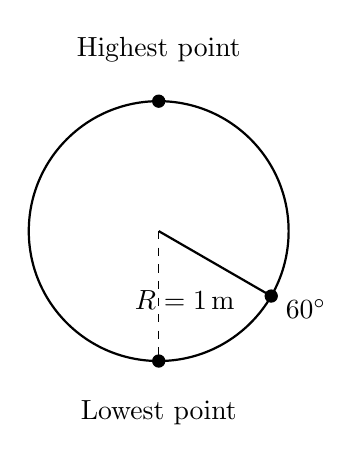
\begin{tikzpicture}[scale=1.1]

% Circle
\draw[thick] (0,0) circle (1.5);

% Lowest and highest points
\filldraw (0,-1.5) circle (2pt);
\filldraw (0,1.5) circle (2pt);

% Radius
\draw[dashed] (0,0) -- (0,-1.5);
\node at (0.3,-0.8) {$R=1\,\text{m}$};

\draw[thick] (0,0) -- (1.299,-0.75);
\filldraw (1.299,-0.75) circle (2pt);
\node at (1.7,-0.9) {$60^\circ$};

% Labels
\node at (0,-2.1) {Lowest point};
\node at (0,2.1) {Highest point};

\end{tikzpicture}
\end{center}

\begin{enumerate}[label=\Alph*)]
\item 16
\item 22
\item 10
\item 28
\end{enumerate}

\item A solid sphere of mass $(2,\text{kg})$ and radius $(0.5,\text{m})$ rolls without slipping down an incline of angle $(30^\circ)$, $(g=10,\text{m/s}^2)$. Using coupled translational and rotational equations with no-slip constraint, determine linear acceleration of centre of mass (in m/s$^2$).

% ===============================
% DIAGRAM FOR QUESTION 13
% Rolling Solid Sphere
% ===============================



\begin{center}
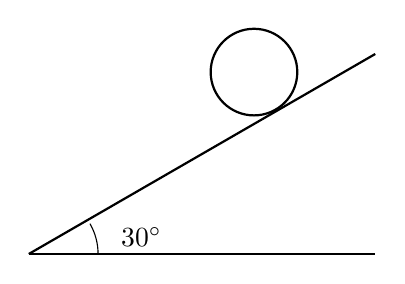
\begin{tikzpicture}[scale=1.1]

% Incline
\draw[thick] (0,0) -- (4,0);
\draw[thick] (0,0) -- (4,2.309);

% Sphere
\draw[thick] (2.6,2.1) circle (0.5);
% Angle
\draw (.8,0) arc (0:30:0.7);
\node at (1.3,0.2) {$30^\circ$};

\end{tikzpicture}
\end{center}

\begin{enumerate}[label=\Alph*)]
\item 3.5
\item 2.8
\item 2.5
\item 4.2
\end{enumerate}

\item A block of mass $(1,\text{kg})$ rests on another block of mass $(4,\text{kg})$; coefficient of friction between them is $(0.5)$, ground is smooth. A horizontal force $(20,\text{N})$ is applied to lower block; $(g=10,\text{m/s}^2)$. Using simultaneous friction constraint and common acceleration condition, determine acceleration of system (in m/s$^2$) assuming no slipping.

% ===============================
% DIAGRAM FOR QUESTION 14
% Two Blocks with Friction
% ===============================



\begin{center}
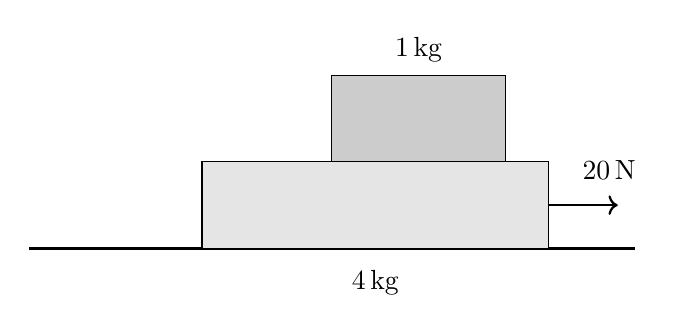
\begin{tikzpicture}[scale=1.1]

% Ground
\draw[thick] (-3,0) -- (4,0);

% Lower block
\draw[fill=gray!20] (-1,0) rectangle (3,1);
\node at (1,-0.4) {$4\,\text{kg}$};

% Upper block
\draw[fill=gray!40] (0.5,1) rectangle (2.5,2);
\node at (1.5,2.3) {$1\,\text{kg}$};

% Force arrow
\draw[->,thick] (3,0.5) -- (3.8,0.5);
\node at (3.7,0.9) {$20\,\text{N}$};

\end{tikzpicture}
\end{center}

\begin{enumerate}[label=\Alph*)]
\item 4
\item 5
\item 3
\item 2
\end{enumerate}

\item A particle of mass $(1,\text{kg})$ moves in a vertical circle of radius $(2,\text{m})$ with speed $(8,\text{m/s})$ at lowest point, $(g=10,\text{m/s}^2)$. Using full energy conservation and radial force equation, determine normal reaction at highest point (in N), if contact is maintained.

\begin{enumerate}[label=\Alph*)]
\item 6
\item 2
\item 10
\item 0
\end{enumerate}

\end{enumerate}

\end{document}